\documentclass[12pt]{beamer}
\usetheme{CambridgeUS}
\usepackage[utf8]{inputenc}
\usepackage[spanish]{babel}
\usepackage{amsmath}
\usepackage{amsfonts}
\usepackage{amssymb}
\usepackage{graphicx}
\author{Kevin García - Alejandro Vargas}
\title{Multicolinealidad}
%\setbeamercovered{transparent} 
%\setbeamertemplate{navigation symbols}{} 
%\logo{} 
%\institute{} 
%\date{} 
%\subject{} 
\begin{document}

\begin{frame}
\titlepage
\end{frame}

%\begin{frame}
%\tableofcontents
%\end{frame}
\begin{frame}
\frametitle{Introducción}
~\\ En esta presentación evaluaremos la presencia de multicolinealidad en el modelo lineal ajustado para los 500 datos seleccionados de la base de datos 'cadata'. Se dará una presentación formal de la multicolinealidad y se mostraran algunas consecuencias que tiene la presencia de este, además, se describirán y se aplicarán distintos métodos para verificar la presencia o ausencia de esta en nuestro modelo lineal ajustado, posteriormente se tratara de solucionar esto, llevando a cabo estimación por PCR(regresión por componentes principales) y finalmente, se concluirá acerca del modelo teniendo en cuenta los resultados de los métodos aplicados y de la estimación por PCR comparada con los estimadores por MCO(mínimos cuadrados ordinarios) .
\end{frame}

\begin{frame}
\frametitle{Modelo planteado}
~\\ El modelo sobre el cuál se va a evaluar la presencia de la multicolinealidad, es el modelo que se planteó en la tarea 1, que pretendía explicar la variable 'Valor mediano de las viviendas' con las variables explicativas 'Ingreso mediano','Edad mediana de la vivienda','Total de habitaciones','Total de dormitorios','Población' y 'Hogares'. El modelo planteado para estas variables, sin hacer transformación ni selección de estas es:

$$ValorMediano =\beta_{0}+\beta_{1}(IngresoMediano)+\beta_{2}(EdadMediana)+\beta_{3}$$
$$(Habitaciones)+\beta_{4}(Dormitorios)+\beta_{5}(Poblacion)+\beta_{6}(Hogares)$$ 
\end{frame}

\begin{frame}
\frametitle{Multicolinealidad}
~\\La multicolinealidad implica una dependencia casi lineal entre los regresores, los cuales son las columnas de la matriz X, por lo que es claro que una dependencia lineal exacta causaría una matriz $X^{T}X$ singular. La presencia de dependencias casi lineales puede influir en forma dramática sobre la capacidad de estimar coeficientes de regresión afectando la precisión de las estimaciones. Cuando existe multicolinealidad en nuestro modelo, el análisis por mínimos cuadrados puede ser totalmente inadecuado.
\end{frame}

\begin{frame}
\frametitle{Posibles causas de la multicolinealidad}
~\\La multicolinealidad se puede dar por cuatro fuentes principales:
\begin{itemize}
\item[1.]El método de recolección de datos que se empleó:Puede originar problemas de multicolinealidad cuando el analista sólo muestrea un subespacio de la región de los regresores definidos.
\item[2.]Especificación del modelo:También se puede inducir la multicolinealidad por la elección del modelo. Por ejemplo,al agregar términos polinomiales a un modelo de regresión se produce un deterioramiento en $X^{T}X$, además, si el rango de X es pequeño, al agregar un término en $X^{2}$ puede producirse una multicolinealidad importante.
\end{itemize}
\end{frame}

\begin{frame}
\frametitle{Posibles causas de la multicolinealidad}
\begin{itemize}
\item[3.]Restricciones en el modelo o en la población:Las restricciones en el modelo o en la población que se muestrea pueden causar multicolinealidad; por ejemplo, supóngase que una empresa eléctrica está investigando el efecto del ingreso familiar $(X_{l})$ y el tamaño de la vivienda $(X_{2})$ sobre el consumo eléctrico residencial.En este ejemplo, una restricción física en la población fue lo que causó este fenómeno: las familias que tienen ingresos mayores en general tienen casas mayores que las familias de menores ingresos, cuando hay restricciones físicas como ésta, habrá multicolinealidad independientemente del método de muestreo que se emplee.
\item[4.]Un modelo sobredefinido:Cuando se tienen mas variables regresoras que observaciones se puede generar un problema de multicolinealidad.
\end{itemize}
\end{frame}


\begin{frame}
\frametitle{Consecuencias de la multicolinealidad}
~\\Una multicolinealidad fuerte entre los regresores del modelo,da como resultado grandes varianzas y covarianzas de los estimadores de coeficientes de regresión por mínimos cuadrados.Esto implica que distintas muestras tomadas con los mismos valores de X podrían ocasionar estimaciones muy diferentes de los parámetros del modelo.
\end{frame}

\begin{frame}
\frametitle{Métodos para detectar multicolinealidad}
~\\Para detectar la multicolinealidad se utilizaran los 4 métodos de diagnostico expuestos en el libro de montgomery, que son los siguientes:
\begin{itemize}
\item[1.]Examen de la matriz de correlación:Una medida muy sencilla de la multicolinealidad es la inspección de los elementos $r_{ij}$ no diagonales en la matriz de correlaciones. Si los regresores $x_{i}$ y $x_{j}$ son casi linealmente dependientes $|r_{ij}|$ será próximo a 1. Para nuestros datos, la matriz de correlaciones es la siguiente:
\end{itemize}
\end{frame}

\begin{frame}
\frametitle{Métodos para detectar multicolinealidad}

\[R=
\left( \begin{array}{cccccc}
 1 & 0.01725 & 0.07903 & -0.18136 & -0.16257 & -0.16049 \\ 
   & 1       & -0.31169& -0.17024 & -0.26517 & -0.14456 \\
   &         & 1       & 0.86207  & 0.85768  & 0.86527 \\
   &         &         & 1        & 0.83406  & 0.98870 \\
   &         &         &          & 1        & 0.85391 \\
   &         &         &          &          & 1
\end{array} \right) \]
~\\La matriz de correlaciones R, nos muestra perfectamente la alta correlación que existe entre las últimas 4 variables regresoras o explicativas (Total de habitaciones, total de dormitorios, población y hogares) , por lo cuál es casi evidente que una o varías de estas sobran en el modelo y pueden ocasionar multicolinealidad.
\end{frame}

\begin{frame}
\frametitle{Métodos para detectar multicolinealidad}
\begin{itemize}
\item[2.]Factores de inflación de varianza:Como la varianza de los j-ésimos coeficientes de regresión es $C_{jj}\sigma^2$ se puede considerar que $C_{jj}$ es el factor en el que aumenta la varianza de $\hat{\beta_{j}}$ debido a dependencias casi lineales entre los regresores.
~\\Entonces se define el factor de inflación de varianza como: 
$$VIF_{j}=C_{jj}=(1-R^2_{j})^{-1}$$
~\\El factor VIF (de variance inflation factor) para cada término del modelo mide el efecto combinado que tienen las dependencias entre los regresores sobre la varianza de ese término. Si hay uno o más VIF grandes, hay multicolinealidad. El criterio dice que si cualquiera de los VIF es mayor que 5 o 10, es indicio de que los coeficientes asociados de regresión están mal estimados debido a la multicolinealidad.
\end{itemize}
\end{frame}

\begin{frame}
\frametitle{Métodos para detectar multicolinealidad}
~\\Los $VIF_{i}$ para este modelo son:
\begin{figure}[!h]
    \begin{center}
        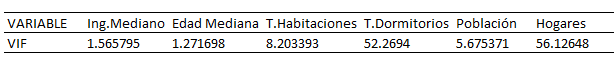
\includegraphics[width=12cm]{imagenes/VIFS.png}
        \label{fig:Densidad}
    \end{center}
\end{figure}
~\\Podemos ver que hay 2 VIF mayores que 5 y 2 VIF mayores que 10, entonces podemos afirmar que los coeficientes de regresión asociados a estas variables están mal estimados debido a la multicolinealidad.
\end{frame}

\begin{frame}
\frametitle{Métodos para detectar multicolinealidad}
\begin{itemize}
\item[3.]Análisis del eigensistema de $X^{T}X$:Los valores propios de $X^{T}X$, por ejemplo $\lambda_{1},\lambda_{2},...,\lambda_{p}$ se pueden usar para medir el grado de multicolinealidad en los datos. Si hay una o más dependencias casi lineales en los datos, una o más de las raíces características será pequeña. Uno o más eigenvalores pequeños implican que hay dependencias casi lineales entre las columnas de X. Algunos analistas prefieren examinar el número de condición de $X^{T}X$, que se define como $k=\frac{\lambda_{max}}{\lambda_{min}}$
~\\En general, si el número de condición es menor que 100, no hay problema grave de multicolinealidad. Los números de condición de 100 a 1 000 implican multicolinealidad de moderada a fuerte, y si k es mayor que 1 000, es indicio de una fuerte multicolinealidad.
\end{itemize}
\end{frame}

\begin{frame}
\frametitle{Métodos para detectar multicolinealidad}
~\\Los indices de condición de la matriz $X^{T}X$ son
~\\$$k_{j}=\frac{\lambda_{max}}{\lambda_{j}} ; j=1,2,...,p$$
~\\La cantidad de indices de condición que son grandes (digamos, $\geq 1000$) es una medida útil de la cantidad de dependencias casi lineales en $X^{T}X$.
~\\Los valores propios para la matriz $X^{T}X=R$ (en forma de correlación) correspondiente a nuestros datos son:
~\\$\lambda_{1}=3.72181333,\lambda_{2}=1.05255886,\lambda_{3}=0.93404888,\lambda_{4}=0.19394997,\lambda_{5}=0.08822446,\lambda_{6}=0.00940450$
\end{frame}

\begin{frame}
\frametitle{Métodos para detectar multicolinealidad}
~\\De aquí, tenemos que $\lambda_{max}=3.72181333$ y $\lambda_{min}=0.00940450$, por lo tanto el número de condición es:
$$k=\frac{\lambda_{max}}{\lambda_{min}}=\frac{3.72181333}{0.00940450}=395.7481344$$
~\\El cuál es demasiado grande, lo que nos indica una multicolinealidad fuerte en nuestro modelo con todas las variables.
~\\Y los indices de condición son:
~\\$$k_{1}=\frac{3.72181333}{3.72181333}=1,k_{2}=\frac{3.72181333}{1.05255886}=3.5359669$$
~\\$$k_{3}=\frac{3.72181333}{0.93404888}=3.9846023$$
\end{frame}

\begin{frame}
\frametitle{Métodos para detectar multicolinealidad}
~\\$$k_{4}=\frac{3.72181333}{0.19394997}=19.189553,k_{5}=\frac{3.72181333}{0.08822446}=42.18573092$$
~\\$$k_{6}=\frac{3.72181333}{0.00940450}=395.7481344$$
~\\Podemos ver que un indice de condición es mayor que 100, lo que nos dice que al menos hay una dependencias fuerte casi lineales en los datos de nuestro modelo (columnas de $X^{T}X$).
\end{frame}

\begin{frame}
\frametitle{Métodos para detectar multicolinealidad}
\begin{itemize}
\item[4.]Determinante de $X^{T}X$ en forma de correlación: Se puede usar el determinante de $X^{T}X$ como índice de colinealidad; ya que la matriz $X^{T}X$ está en forma de correlación, el intervalo de posibles valores del determinante es $0\leq |X^{T}X| \leq 1$. Si $|X^{T}X| = 1$, los regresores son ortogonales, mientras que si $|X^{T}X|=0$, hay una dependencia lineal exacta entre ellos. El grado de multicolinealidad se agrava a medida que $|X^{T}X|$ tiende a cero. Si bien esta medida de multicolinealidad es fácil de aplicar, no proporciona información alguna sobre el origen de la multicolinealidad.
~\\Para nuestro caso el determinante de la matriz de correlaciones $X^{T}X$ es:$|X^{T}X|=|R|=0.0005888233$
~\\Por lo cual podemos afirmar que hay una multicolinealidad grave en nuestro modelo.
\end{itemize}
\end{frame}

\begin{frame}
\frametitle{Regresión por componentes principales (PCR)}
~\\Los coeficientes de regresión se pueden obtener por un procedimiento denominado regresión por componentes principales. Sea la forma canónica del modelo:
$$y=Z\alpha+\epsilon$$
~\\Donde $Z=XT$, $\alpha=T'\beta$,  $T'X'XT=Z'Z=A$ 
~\\Y $A=diag(\lambda_{1},\lambda_{2},...,\lambda_{p})$ es una matriz diagonal de tamapo p x p de los valores propios de $X'X$ y T es una matriz ortogonal cuyas columnas son los vectores propios asociados a los valores propios $\lambda_{1},\lambda_{2},...,\lambda_{p}$. Las columnas de Z, definen un nuevo conjunto de regresores ortogonales, como:
$$Z=[Z_{1},Z_{2},...,Z_{p}]$$ Se llaman componentes principales
\end{frame}

\begin{frame}
\frametitle{Regresión por componentes principales (PCR)}
~\\Entonces, el estimador de $\hat{\alpha}$ por minimos cuadrados es
$$\hat{\alpha}=(Z'Z)^{-1}Z'y= A^{-1}Z'y$$
~\\Y la matriz de covarianzas de $\hat{\alpha}$ es 
$$Var(\hat{\alpha})=\sigma^2 (Z'Z)^{-1}=\sigma^2 A^{-1}$$
~\\El método de regresión por componentes principales combate a la multicolinealidad,
al usar en el modelo menos componentes que el conjunto completo de componentes principales. Para obtener el estimador de componentes principales, se supone que los regresores están ordenados por valores propios decrecientes, $\lambda_{1}\geq\lambda_{2}\geq...\geq\lambda_{p}>0$.
\end{frame}

\begin{frame}
\frametitle{Regresión por componentes principales (PCR)}
~\\Supóngase que los últimos s eigenvalores de éstos son aproximadamente iguales a cero. En la regresión por componentes principales, se eliminan los componentes principales que correspondan a eigenvalores cercanos a cero, y se aplican los mínimos cuadrados a los componentes restantes. Esto es,
$$\hat{\alpha_{PC}}=B\hat{\alpha}$$
donde $b_{1}=b_{2}=...=b_{p-s}=1$, y $b_{p-s+1}=b_{p-s+2}=...=b_{p}=0$.Así, el estimador de componentes principales es
$$\hat{\alpha_{PC}}=\left[\begin{matrix}
\hat{\alpha_{1}} & \hat{\alpha_{2}} & \cdots & \hat{\alpha_{p-s}} & | & 0 & 0 & \cdots & 0
\end{matrix}\right]$$ 
\end{frame}

\begin{frame}
\frametitle{Regresión por componentes principales (PCR)}
~\\ o, en términos de los regresores normalizados,
$$\hat{\beta}_{PC}=T\hat{\alpha}_{PC}=\sum\limits_{j=1}^{p-1}\lambda_{j}^{-1}t'_{j}X'yt_{j}$$
~\\Para hacer uso de la regresión por componentes principales en nuestro modelo, se comienza con la transformación lineal $Z=XT$ que transforma los regresores estandarizados originales en un conjunto ortogonal de variables (los componentes principales). Los valores propios $\lambda_{j}$ y la matriz T para los 500 datos seleccionados de la base de datos 'cadata' se muestran en la siguiente tabla.La matriz T indica la relación entre Z y los regresores estandarizados. 
\end{frame}

\begin{frame}
\frametitle{Regresión por componentes principales (PCR)}
~\\Por ejemplo, la relación entre $Z_{1}$ y los regresores estandarizados es 
$$z_{1}=-0.0785x_{1}-0.1609x_{2}+0.4854x_{3}+0.4987x_{4}+0.4831x_{5}+0.5002x_{6}$$
\begin{figure}[!h]
    \begin{center}
        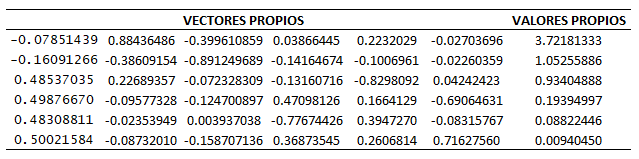
\includegraphics[width=12cm]{imagenes/vec.png}
        \label{fig:Densidad}
    \end{center}
\end{figure}
\end{frame}

\begin{frame}
\frametitle{Regresión por componentes principales (PCR)}
~\\Y, el estimador de $\alpha$ es:
 $$\hat{\alpha}=A^{-1}Z'y=\left[\begin{matrix}
 -0.02697939 \\ 
 0.16597000 \\ 
 -0.64338425 \\ 
 0.75560789 \\ 
 -0.28640901 \\ 
 0.81285787
 \end{matrix}\right]$$
\end{frame}

\begin{frame}
\frametitle{Regresión por componentes principales (PCR)}
~\\Podemos ver que hay 3 valores propios muy cercanos a cero, por lo que esos no se tendrán en cuenta y nos quedaremos con las componentes principales correspondientes a los otros tres valores propios, entonces:
$$\hat{\alpha_{PC}}=\left[\begin{matrix}
 -0.02697939 \\ 
 0.16597000 \\ 
 -0.64338425 \\ 
0 \\ 
 0 \\ 
 0
 \end{matrix}\right]$$
\end{frame}

\begin{frame}
\frametitle{Regresión por componentes principales (PCR)}
~\\Y, los betas estimados con tres componentes principales son:
$$\hat{\beta}_{PC}=T\hat{\alpha}_{PC}=\left[\begin{matrix}
 0.40599964 \\ 
 0.51367772 \\ 
 0.07109743 \\ 
 0.05087868 \\ 
 -0.01947330 \\ 
 0.07412164
 \end{matrix}\right]$$
\end{frame}

\begin{frame}
\frametitle{Regresión por componentes principales (PCR)}
~\\En la siguiente tabla vemos los coeficientes correspondientes a MCO y PCR utilizando tres componentes principales:
\begin{figure}[!h]
    \begin{center}
        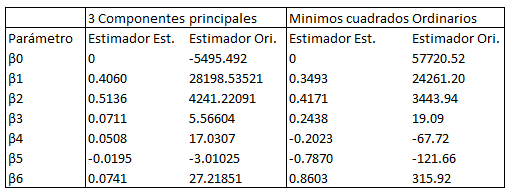
\includegraphics[width=12cm]{imagenes/com.png}
        \label{fig:Densidad}
    \end{center}
\end{figure}
\end{frame}

\begin{frame}
\frametitle{Comparación de modelos y conclusión}
\begin{center}
\begin{tabular}{|ccc|}
\hline 
 & $R^2$ & $\sigma^2$ \\ 
\hline 
MCO & 0.5425316 & 6724487923 \\ 
\hline 
PCR & 0.4183462 & 8549932422 \\ 
\hline 
\end{tabular} 
\end{center}
~\\La regresión PCR resuelve el problema de multicolinealidad reduciendo el numero de componentes principales que el modelo completo o regresión por mínimos cuadrados utiliza, sin embargo la varianza de este método aumentó, lo que es un punto en contra, aun así es una buena alternativa para solucionar este problema. También apreciamos que el $R^2$ disminuyó considerablemente, esto tal vez es debido a que se quitan componentes que explican poco sobre la variabilidad del modelo y esto hace que el $R^2$ disminuya en proporción a cuantos componentes se eliminan del modelo.
\end{frame}



\end{document}